\chapter{Methodology}
\label{cp:methodology}

\section{Apparatus}\label{sec:apparatus}

An airfoil is positioned in the wind tunnel test chamber as seen in \autoref{fig: AirfoilTestSection_forward}. The airfoil contains pressure taps around its surface connected to three Scanivalve pressure transducers. \autoref{fig: scanivalve_side} shows the tubes connecting the airfoil pressure taps to the Scanivalve pressure transducers. A computer with data acquisition software collects measurements from the pressure transducers and stores the data in \verb|.csv| files.

\begin{figure}[htpb]
    \centering
    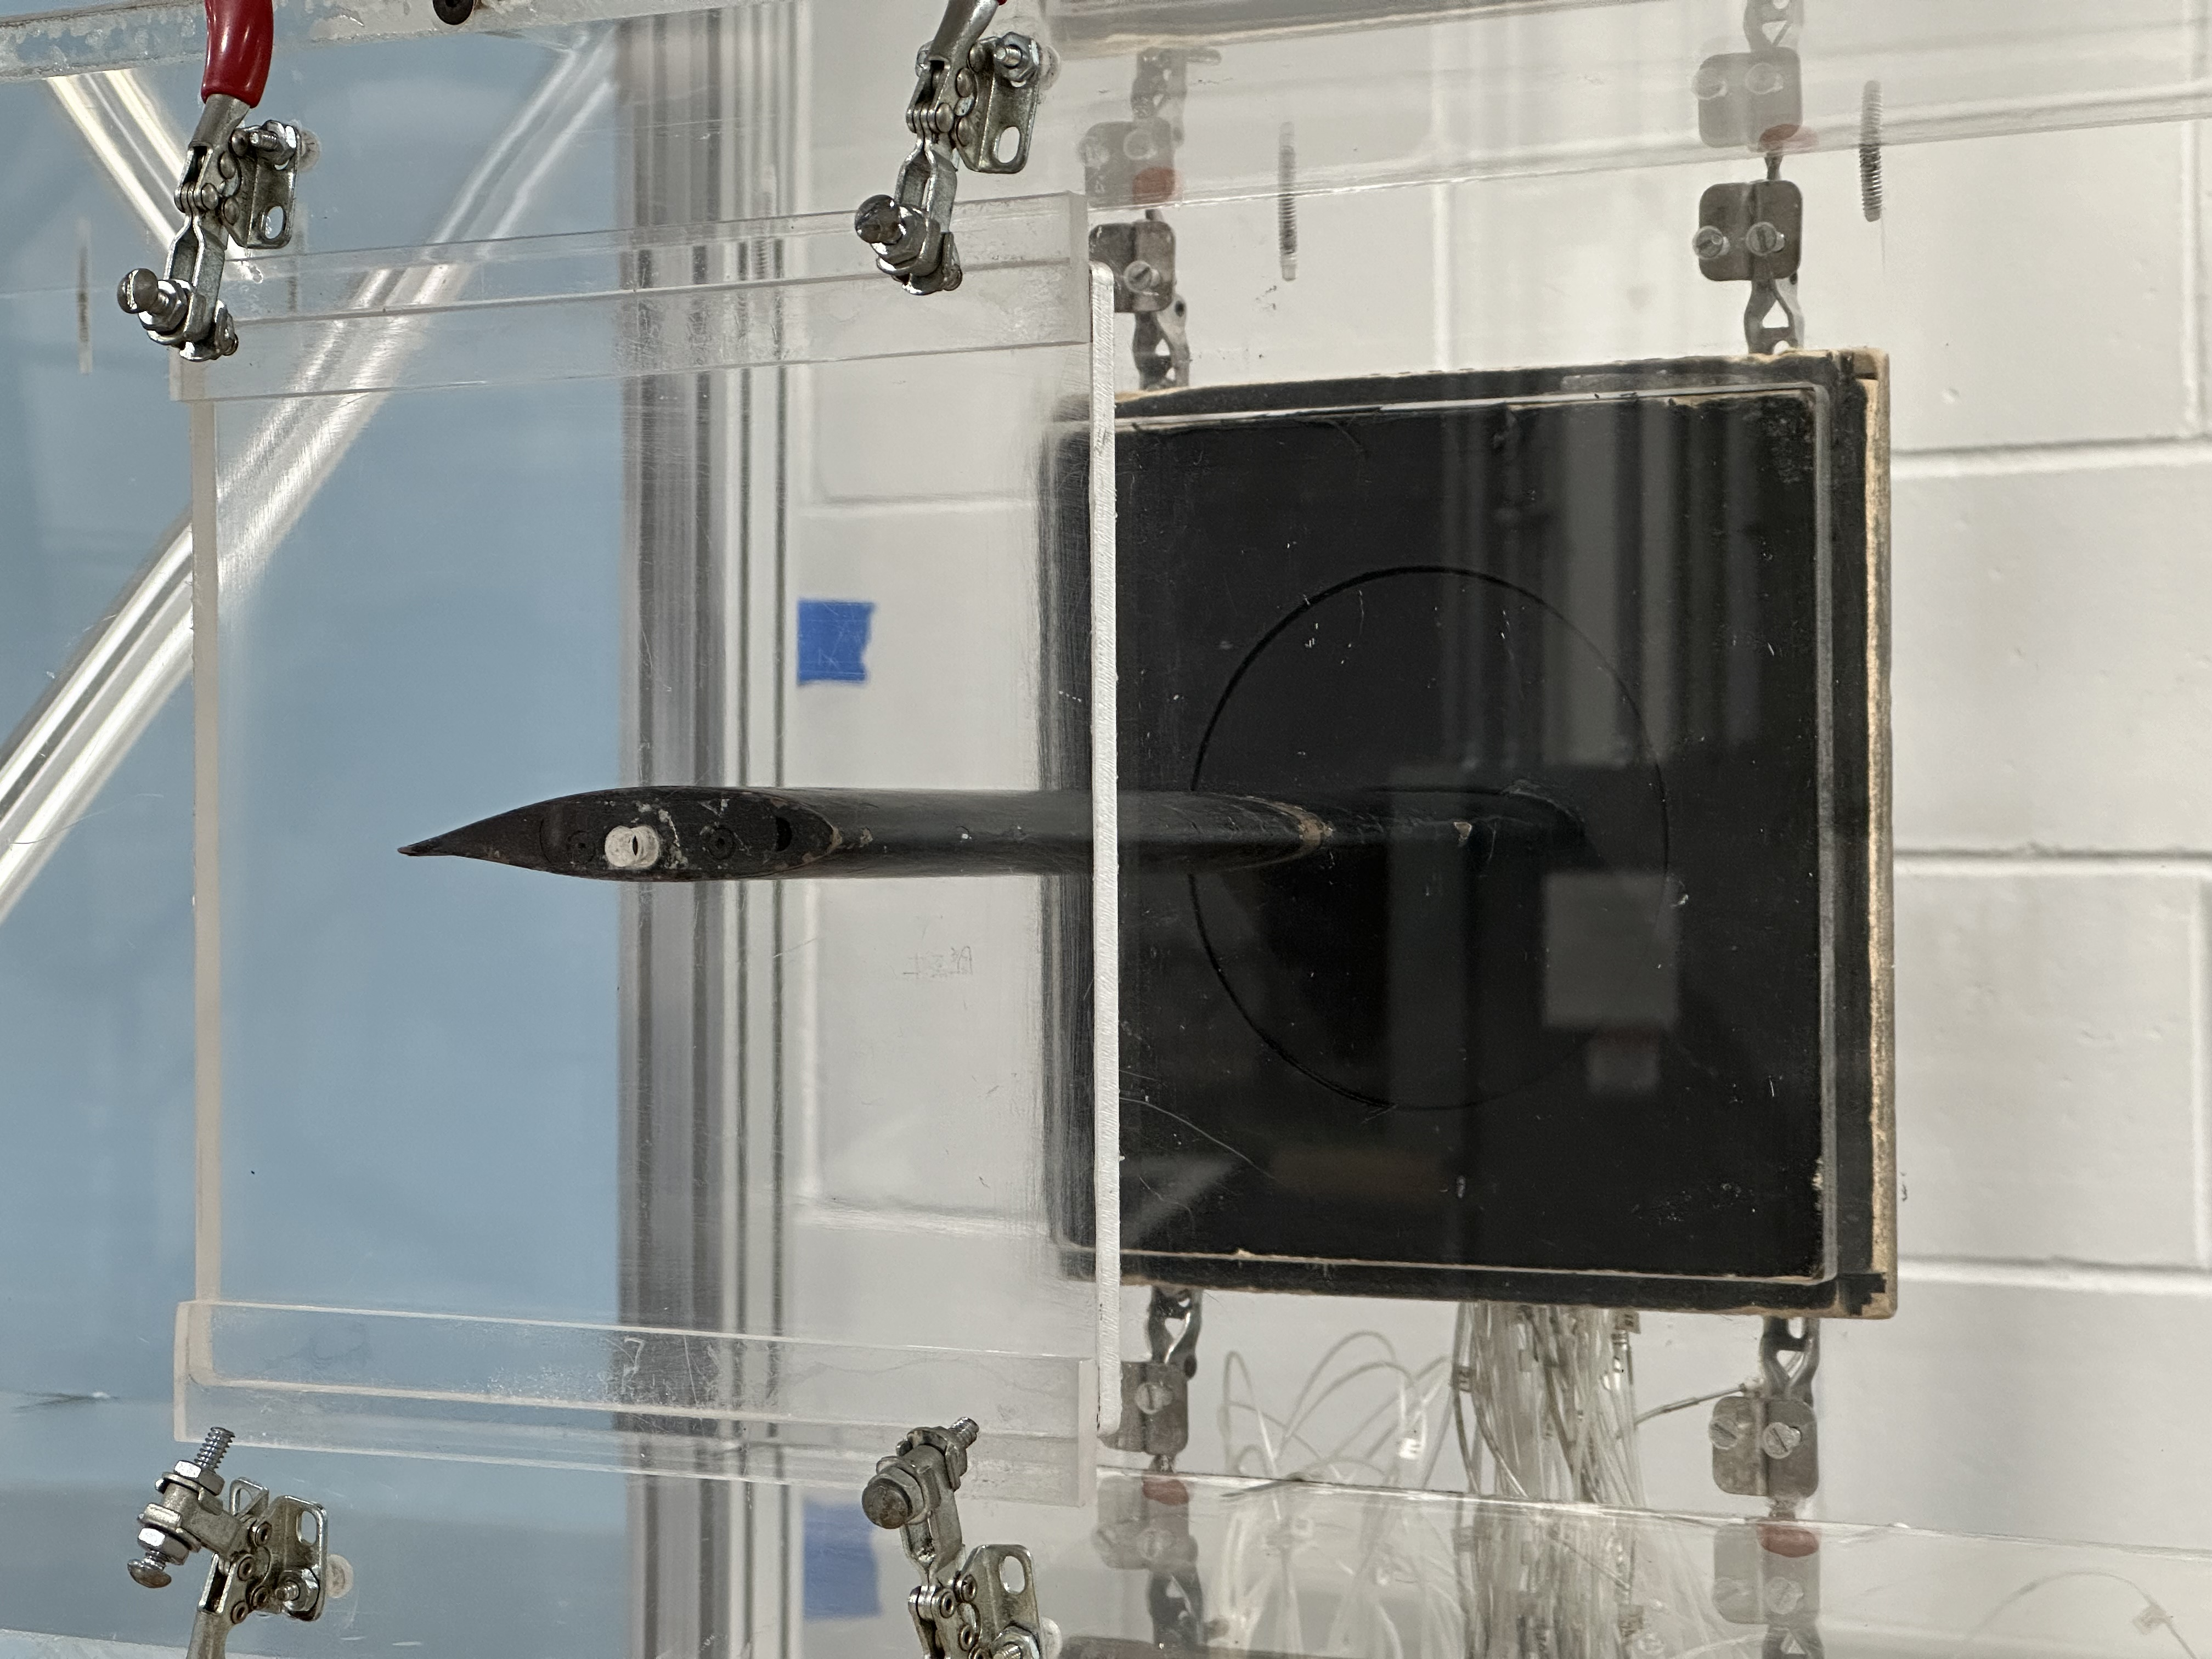
\includegraphics[width=0.75\linewidth]{Figures/IMG_3160.jpeg}
    \caption[Image of Airfoil in Test Section.]{Image of Airfoil in Test Section.}
    \label{fig: AirfoilTestSection_forward}
\end{figure}

\begin{figure}[htpb]
    \centering
    \includegraphics[width=0.75\linewidth]{Figures/IMG_3162.jpeg}
    \caption[Image of the Scanivalve tester next to the test section.]{Image of the Scanivalve tester next to the test section.}
    \label{fig: scanivalve_side}
\end{figure}

\newpage
\section{Procedure}\label{sec:procedures}

\begin{enumerate}
    \item Determine the correct motor frequency to use for a wind tunnel velocity of \qtyrange{10}{15}{\meter\per\second}.
    \item Verify the connections to the three Scanivalve pressure transducers.
    \item Using the data acquisition software, calibrate the three Scanivalve pressure transducers.
    \item Set the wind tunnel to \qtyrange{10}{15}{\meter\per\second}.
    \item Set the \acrshort{aoa} to \qty{-4}{\degree}.
    \item Using the data acquisition software, start a file, press the ``Start'' button, press the ``Close File'' button, and then change the \acrshort{aoa} according to the lab manual. \label{it:data_aq}
    \item Repeat \autoref{it:data_aq} for \acrshort{aoa} \qtylist{-4;0;4;6;8;10;12;14;16}{\degree}. \label{it:repeat}
    \item Repeat \autoref{it:data_aq} and \autoref{it:repeat} as many times as time allows.
    \item Save the data to a flash drive for post-lab analysis.
\end{enumerate}

\section{Derivations}\label{sec:derivations}

The surface of the airfoil can be broken into \gls{N} panels. For a generic, $i$th panel, the panel boundaries come from the $i$th and $i+1$th taps at (\gls{x_i},\gls{y_i}) and $(x_{i+1},y_{i+1})$. This expression is valid for all the panels except the \gls{N}th panel, which is bounded by a fictitious $N+1$ tap that takes on the value of the first tap.

To determine the pressure acting on each panel of the airfoil—which is the average of the pressure between two pressure taps—we use

\begin{equation}\label{eq:p_def}
    \begin{cases}
        p_{i+1/2}=\frac{1}{2}\left(p_i + p_{i + 1}\right) \\
        p_{N+1/2}=\frac{1}{2}\left(p_N + p_1\right)
    \end{cases}
\end{equation}

\noindent where \gls{p_(i+1/2)} is the averaged pressure at the $i$th panel and \gls{p_i} is the pressure measured at the $i$th pressure tap.

To find the lift, drag, and moment forces over the airfoil, we use trapezoidal integration. Before we can integrate, we must define

\begin{equation}\label{eq:coord_def}
    \begin{cases}
        \Delta x_i = x_{i+1} - x_i,&\quad \Delta y_i=y_{i+1}-y_i \\
        \Delta x_N = x_1 - x_N,&\quad\Delta y_N = y_1 - y_N
    \end{cases}
\end{equation}

\noindent where \gls{Delta x_i} and \gls{Delta y_i} are the distances between the $i$th pressure tap and the $i+1$th pressure tap in the $x$ and $y$ coordinate systems respectively and \gls{x_i} and \gls{y_i} is the location of the $i$th pressure tap in the $x$ and $y$ coordinate system. \autoref{fig:trapezoid} shows the generalized trapezoid used to integrate.

\begin{figure}[htpb]
    \centering
    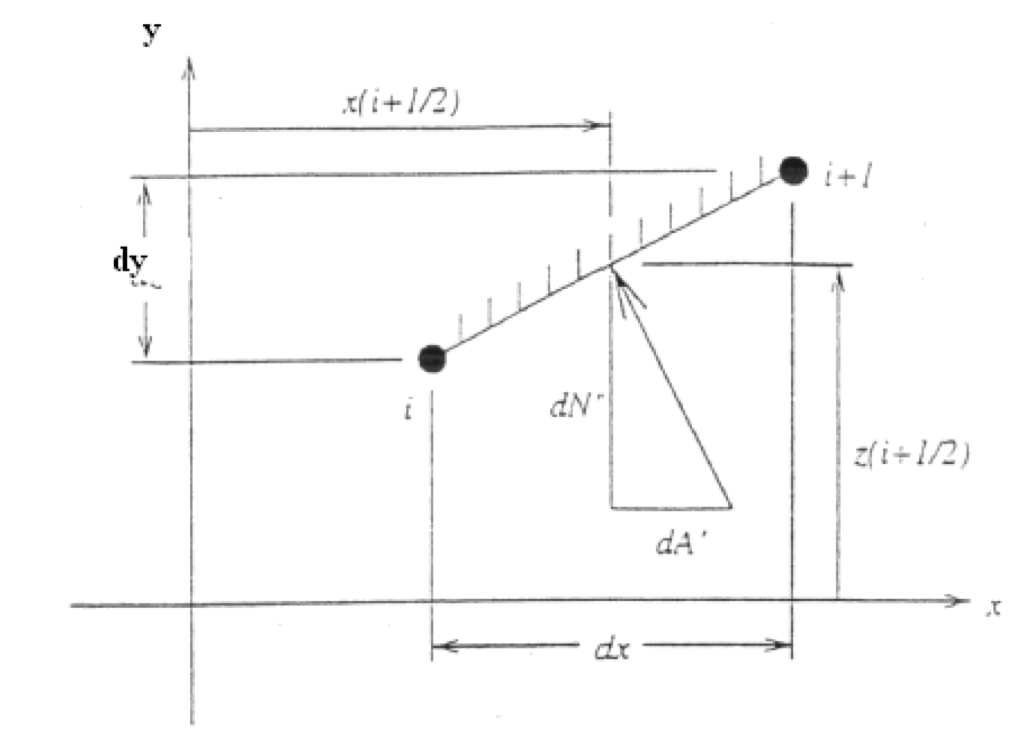
\includegraphics[width=0.75\linewidth]{Figures/trapezoid.png}
    \caption[A diagram of the trapezoidal integration setup]{A diagram of the trapezoidal integration used to calculate \gls{C_L}, \gls{C_D}, and \gls{C_M} \citep{lab5-manual}.}
    \label{fig:trapezoid}
\end{figure}

Using \autoref{eq:p_def} and \autoref{eq:coord_def}, we can derive the following force per unit span components:

\begin{align}
    \delta N'_i &= p_{i+1/2} \Delta x_i \\
    \delta A'_i &= -p_{i+1/2} \Delta y_i \\
    \delta M'_{LE,i} &= -\left(p_{i+1/2} \Delta x_i\right)x_{i+1/2} - \left(p_{i+1/2} \Delta y_i\right)y_{i+1/2}
\end{align}

\noindent where \gls{Del N'_i} is the normal component of pressure on the $i$th panel, \gls{Del A'_i} is the axial component of pressure on the $i$th panel, \gls{Del M'_LE,i} is the aerodynamic moment force on the $i$th panel, and $x_{i+1/2}$ and $y_{i+1/2}$ are defined as

\begin{align}
    x_{i+1/2}&=\frac{1}{2}\left(x_i+x_{i+1}\right) \\
    y_{i+1/2}&=\frac{1}{2}\left(y_i+y_{i+1}\right)
\end{align}

Once each component of the aerodynamic forces is calculated, we sum the component to find the total aerodynamic forces per unit span as shown blow:

\begin{align}
    N'&=\sum_{i=1}^N\delta N'_i \\
    A'&=\sum_{i=1}^N\delta A'_i \\
    M'_{LE}&=\sum_{i=1}^N\delta M'_{LE,i}
\end{align}

\noindent where \gls{N'} and \gls{A'} are the sums of the pressure forces in the normal and axial directions respectively and \gls{M'_LE} is the total moment caused by the pressure forces on the airfoil. We can use \gls{N'} and \gls{A'} to find the lift and drag forces per unit span, \gls{L'} and \gls{D'}, respectively:

\begin{align}
    L' &= N'\cos{\alpha} - A'\sin{\alpha} \\
    D' &= N'\sin{\alpha} + A'\cos{\alpha}
\end{align}

\noindent where \gls{alpha} is the angle of attack.

To find the coefficients of lift, drag, and moment—\gls{C_L}, \gls{C_D}, and \gls{C_M}, respectively—we must also calculate the dynamic pressure, $q=\frac{1}{2}\rho v^2$. Then, using the forces per unit span we derived above and dividing them by the dynamic pressure, we find

\begin{align}
    C_l &= \frac{L'}{q} \\
    C_d &= \frac{D'}{q} \\
    C_m &= \frac{M'_{LE}}{q}
\end{align}

Finally, we wrote a \acrfull{matlab} script to visualize the data into graphs (see \autoref{sec:code}).